\documentclass[14pt, a4paper]{extreport}
\usepackage[utf8]{inputenc}
\usepackage[russian]{babel}
\usepackage[top=20pt,bottom=70pt]{geometry}
\usepackage{amssymb}
\usepackage{amsmath}
\usepackage{graphicx}
\usepackage[nottoc]{tocbibind}
\renewcommand*\rmdefault{cmr}
\graphicspath{{.}}
\usepackage[left=2cm,right=2cm,bottom=3cm,top=2cm]{geometry}


\DeclarePairedDelimiter{\abs}{\lvert}{\rvert}

\linespread{1.25}

\begin{document}

\thispagestyle{empty}

\begin{center}
\ \vspace{-3cm}

\includegraphics[width=0.5\textwidth]{msu.eps}\\
{Московский государственный университет имени М.В.~Ломоносова}\\
Факультет вычислительной математики и кибернетики\\
Кафедра алгоритмических языков

\vspace{5cm}

{\Large Кошовец Олег Игоревич}

\vspace{1cm}

{\Large\bfseries
Разложение матрицы полиномов от нескольких переменных в произведение элементарных матриц\\}

\vspace{1cm}

{\large ВЫПУСКАНЯ КВАЛИФИКАЦИОННАЯ РАБОТА}
\end{center}

\vfill

\begin{flushright}
  \textbf{Научный руководитель:}\\
  Профессор\\
  С.А.Абрамов
\end{flushright}

\vfill


\begin{center}
Москва, 2018
\end{center}
\newpage

	\chapter{Введение}
		Иногда при решении систем дифференциальных уравнений можно установить ряд
		свойств решений, исследуя только матрицы дифференциальных операторов,
		которые описывают систему.
		\\\\
		Условие разложимости матрицы в произведение элементарных матриц является
		признаком голоморфности решений.
		Однако в ряде случаев задача о матрицах дифференциальных операторов
		может быть сведена к задаче о полиномиальных матрицах.
		\section{Постановка задачи}
		В данной работе исследуются матрицы полиномов от одной переменной,
		и способы их разложения в произведение элементарных матриц.
		Конечная задача - написать программу, производящую разложение
		исходной матрицы в произведение элементарных.
	\newpage
	\chapter{Системы дифференциальных уравнений}
		\section{Задача Коши}
		Пусть $A(x;D) = (a_{ij}(x;D))_{1 \leq i, j \leq N}$ - система обыкновенных
		дифференциальных операторов с голоморфными коэффициентам из $\Omega \subset C$,
		где $D = d/dx$. Пусть $T = (t_1,...,t_n)$ - неотрицательные целые числа. \\
		Тогда можно поставить задачу Коши $(A(x;D), T)$ следующим образом:
		\begin{center}
			$\sum\limits_{j=1}^N a_{ij}(x;D)u_j(x) = f_i(x), \ \ \ \ 1 \leq i \leq N,$
		\end{center}
		\begin{center}
			$D^ku_i(x_0) = w_{i, k} \in C,\ \ \ \ 0 \leq k < t_i, \ \ \ \ 1 \leq i \leq N, $
		\end{center}
		где $x_0 \in \Omega$\\\\
		\section{Свойства решений}
		В работе \cite{miyake} Масатаке Мияке приведены и доказаны теоремы, согласно которым система
		имеет голоморфные решения в каждой точке $x_0 \in \Omega$ тогда и только тогда,
		когда система дифференциальных операторов $A(x;D)$ может быть разложена
		в произведение элементарных матриц. \\\\
		Разложение произвольной системы дифференциальных операторов в произведение
		элементарных матриц - очень нетривиальная задача. Мною рассматривалось упрощение
		этой задачи: разложить матрицу полиномов от одной переменной в произведение
		элементарных матриц.
	\newpage
	\chapter{Канонический вид матрицы}
		Пусть матрица $A$ - матрица, состоящая из элементов некоторого кольца
		\[
		\begin{bmatrix}
			a_{11} & a_{12} & \dots & a_{1n} \\
			a_{21} & a_{22} & \dots & a_{2n} \\
			\vdots & \vdots & \ddots & \vdots \\
			a_{m1} & a_{m2} & \dots & a_{mn}
		\end{bmatrix}
		\]
		\section{Канонический диагональный вид}
		Матрица из элементов некоторого кольца называется
		канонической диагональной, если она имеет вид
		\[
		\begin{bmatrix}
			a_{1} & 0 & \dots & 0 & 0 & \dots & 0 \\
			0 & a_{2} & \dots & 0 & 0 & \dots & 0 \\
			\dots & \dots & \dots & \dots & \dots & \dots & \dots \\
			0 & 0 & \dots & a_{s} & 0 & \dots & 0 \\
			0 & 0 & \dots & 0 & 0 & \dots & 0 \\
			\dots & \dots & \dots & \dots & \dots & \dots & \dots \\
			0 & 0 & \dots & 0 & 0 & \dots & 0
		\end{bmatrix}
		\]
		где элементы $a_i$ делятся без остатка на элементы $a_{1..i-1}$
		\section{Элементарные преобразования матриц}
		К элементарным преобразованиям матриц относят следующие
		\begin{enumerate}
			\item Перестановка двух строк или двух столбцов
			\item Умножение строки или столбца на некоторый, отличный от нуля,
			элемент кольца
			\item Прибавление к строке или столбцу другой строки или, соответсвтенно,
			столбца, домноженный на некоторый элемент кольца
		\end{enumerate}
		\section{Алгоритм приведения}
		В\ "Теории матриц"\ \cite{gantmaher} Гантмахер изложил алгоритм приведения матрицы
		к каноническому диагональному виду, использующий только элементарные
		преобразования матриц. Алгоритм состоит из нескольких частей.
		\begin{enumerate}
			\item Выделить в матрице элемент наименьшей степени и
			с помощью перестановок строк и столбцов сделать его элементом $a_{11}$
			\[
			\begin{bmatrix}
				a_{11} & a_{12} & \dots & a_{1n} \\
				a_{21} & a_{22} & \dots & a_{2n} \\
				\vdots & \vdots & \ddots & \vdots \\
				a_{m1} & a_{m2} & \dots & a_{mn}
			\end{bmatrix}
			\]
			\item Последовательно вычесть из строк $2..m$ первую строку,
			домноженную на $q_{s1}$, где $a_{s1} = a_{11}q_{s1} + r_{s1}$, получив
			\[
			\begin{bmatrix}
				a_{11} & a_{12} & \dots & a_{1n} \\
				r_{21} & r_{22} & \dots & r_{2n} \\
				\vdots & \vdots & \ddots & \vdots \\
				r_{m1} & r_{m2} & \dots & r_{mn}
			\end{bmatrix}
			\]
			\item Если среди $r_{21..m1}$ есть элементы, не равные тождественно
			нулю, то алгоритм заново применяется к полученной матрице. В итоге
			получаем матрицу вида
			\[
			\begin{bmatrix}
				a_{11} & a_{12} & \dots & a_{1n} \\
				0 & a_{22} & \dots & a_{2n} \\
				\vdots & \vdots & \ddots & \vdots \\
				0 & a_{m2} & \dots & a_{mn}
			\end{bmatrix}
			\]
			\item По аналогии с пунктом 2 поступаем со столбцами, получая матрицу вида
			\[
			\begin{bmatrix}
				a_{11} & r_{12} & \dots & r_{1n} \\
				0 & a_{22} & \dots & a_{2n} \\
				\vdots & \vdots & \ddots & \vdots \\
				0 & a_{m2} & \dots & a_{mn}
			\end{bmatrix}
			\]
			\item Если среди $r_{12..1n}$ есть элементы, не равные тождественно
			нулю, то алгоритм заново применяется к полученной матрице, начиная
			с пункта 4. В итоге получаем матрицу вида
			\[
			\begin{bmatrix}
				a_{11} & 0 & \dots & 0 \\
				0 & a_{22} & \dots & a_{2n} \\
				\vdots & \vdots & \ddots & \vdots \\
				0 & a_{m2} & \dots & a_{mn}
			\end{bmatrix}
			\]
			\item Алгоритм применяется к $(a_{22}..a_{mn})$ подматрице полученной матрицы.
			На выходе получаем каноническую диагональную матрицу.
		\end{enumerate}
		\newpage
		\section{Элементарные матрицы}
			Каждой элементарной операции над матрицей $A$ можно сопоставить матрицу $S$,
			которая при умножении на исходную матрицу слева или справа выполняет нужное
			преобразование. Действия над строками выполняются с помощью умножения слева
			$S*A$, а операции над столбацми - справа $A*S$. Такие матрицы называются
			элементарными. \\ Любую последовательнось элементарных преобразований можно
			выполнить с помощью последовательного умножения исходной матрицы с нужной
			стороны на соответствующие элементарные матрицы.
	\chapter{Разложение матрицы полиномов}
		Используя алгоритм из Гантмахера, можно привести матрицу к каноническому виду с
		помощью элементарных преобразований. Из этого следует, что из канонического
		вида некоторой матрицы можно восстановить ее исходный вид, проведя обратные
		элементарные преобразования в обратном порядке. Таким образом, переделав
		алгоритм из Гантмахера под нашу конкретную задачу, получаем
		\section{Алгоритм разложения}
		Пусть есть исходная матрица $A$ размера $m*n$
		\[
		\begin{bmatrix}
			a_{11} & a_{12} & \dots & a_{1n} \\
			a_{21} & a_{22} & \dots & a_{2n} \\
			\vdots & \vdots & \ddots & \vdots \\
			a_{m1} & a_{m2} & \dots & a_{mn}
		\end{bmatrix}
		\]
		Пусть матрица $K$ - канонический вид матрицы $A$
		\[
		\begin{bmatrix}
			a_{1} & 0 & \dots & 0 & 0 & \dots & 0 \\
			0 & a_{2} & \dots & 0 & 0 & \dots & 0 \\
			\dots & \dots & \dots & \dots & \dots & \dots & \dots \\
			0 & 0 & \dots & a_{s} & 0 & \dots & 0 \\
			0 & 0 & \dots & 0 & 0 & \dots & 0 \\
			\dots & \dots & \dots & \dots & \dots & \dots & \dots \\
			0 & 0 & \dots & 0 & 0 & \dots & 0
		\end{bmatrix}
		\]
		Тогда
		\begin{equation*}
			(\prod\limits_{i=1}^{q}L_{i})A(\prod\limits_{j=1}^{r}R_{j}) = K
		\end{equation*}
		где $L_{i},R_{j}$ - элементарные матрицы, приводящие исходную матрицы
		к каноническому виду.\\
		Учитывая, что
		\begin{equation*}
			K = (\prod\limits_{l=1}^{s}M_{l})E
		\end{equation*}
		где $M_{l}$ - матрицы, описывающие умножения строки на элемент кольца,а $E$ -
		матрица $m*n$, состоящая из единичной матрицы размера $r*r, r=min(m,n)$
		и нулевой матрицы, можно записать выражение:
		\begin{equation*}
			A =
			(\prod\limits_{i=1}^{q}L_{q-i}^{-1})
			(\prod\limits_{l=1}^{s}M_{l})
			E
			(\prod\limits_{j=1}^{r}R_{r-j}^{-1})
		\end{equation*}
		где матрицы $L_{i}^{-1},R_{j}^{-1},M_{l}$ элементарные.
		\section{Модификация алгоритма}
		Можно заметить, что матрица $S$
		\[
		\begin{bmatrix}
			x^{100} - 1 & 0 & 0 \\
			0 & x & a(x)_{23} \\
			0 & a(x)_{32} & a(x)_{33}
		\end{bmatrix}
		\]
		по алгоритму из Гантмахера должна быть приведена в матрице
		\[
		\begin{bmatrix}
			x & 0 & a(x)_{23} \\
			0 & x^{100} - 1 & 0 \\
			a(x)_{32} & 0 & a(x)_{33}
		\end{bmatrix}
		\]
		а только после этого в ней можно будет упростить первые столбец и строку. При
		этом есть шанс, что для полученной подматрицы элементы тоже сначала придется
		менять местами, а только после этого действовать дальше. При этом на выходе
		может оказаться, что полученная матрица не будет канонической диагональной, так
		как диагональные элементы не будут делиться друга на друга без остатка.\\\\
		Однако для исходной матрицы $S$ перестановки строк можно было не производить
		и сразу перейти к работе с подматрицей, исключив таким образом из итогового
		разложения несколько элементарных матриц, тем самым уменьшив его длину.
		\section{Применимость алгоритма}
			Алгоритм раскладывает любую квадратную невырожденную матрицу в произведение
			элементарных матриц. Также любую прямоугольную матрицу $m*n$ ранга $r=min(m,n)$
			алгоритм раскладывает в произведение матриц, где все кроме одной являются
			элементарными.
	\chapter{Реализация}
		Предложенный выше алгоритм был реализован в системе компьютерной алгебры Maple.
		\section{Оптимизации}
		Алгоритм был оптимизирован с помощью улучшений, описанных выше.\\
		Также была улучшена логика нахождения обратной матрицы: обратные матрицы
		создавались сразу и укладывались в список в обратном порядке, в то время как
		матрицы для построения канонического вида не строились вообще.
		\section{Пример}
		На рисунке представлен пример работы готовой программы.\\
		\begin{center}
			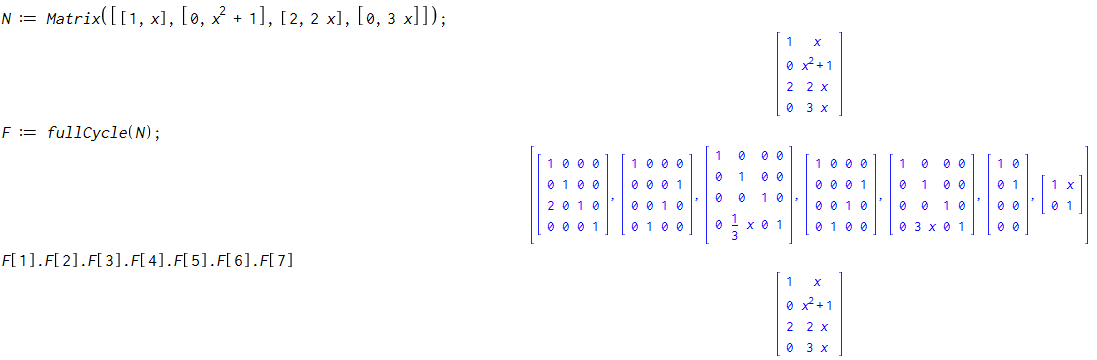
\includegraphics[width=\textwidth]{example.png}
		\end{center}
	\chapter{Итоги}
	\section{Результаты}
	\begin{enumerate}
		\item Изучена работа \cite{miyake} Мисатаке Мияке, сформулирована задача на ее основе
		\item Изучен и переделан алгоритм, представленный в\ "Теории Матриц"\ Гантмахера \cite{gantmaher}
		\item Модифицирован переделанный алгоритм
		\item Изучена система компьютерной алгебры Maple
		\item Реализована программа, производящая разложения матрицы полиномов в
		произведение элементарных матриц
		\item Изучена и освоена верстка в LaTeX
	\end{enumerate}
	\section{Дальнейшие планы}
	\begin{enumerate}
		\item Изучить работы по работе с полиномами от нескольких переменных
		\item Модифицировать текущую программу для работы с матрицами полиномов
		от нескольких переменных
	\end{enumerate}
	Результаты этой научной работы потенциально могут быть использованы
	для решения задач, сформулированных в работе \cite{miyake} Мияке.
	\begin{thebibliography}{5}
		\bibitem{gantmaher}
			Ф.Р.Гантмахер
			\textit{"Теория матриц"}
			Издательство “Наука” 1966
		\bibitem{miyake}
			M.Miyake
			\textit{“Remarks on the formulation of the Cauchy problem 
			for general system of ordinary differential equations”}
			Tohoku Math. Journal 1979
		\bibitem{maple}
			M.Monogan
			\textit{“Maple 9. Introductory Programming Guide”}
			ISBN 1-894511-43-3
		\bibitem{maplesoft}
			\textit{Maplesoft.com}
		\bibitem{mapleprimes}
			\textit{Mapleprimes.com}
	\end{thebibliography}
\end{document}
